\documentclass[10pt]{beamer}

\usetheme[progressbar=frametitle]{metropolis}

\usepackage{booktabs}
\usepackage[scale=2]{ccicons}

\usepackage{graphicx}
\usepackage[outdir=./img/]{epstopdf}
\epstopdfsetup{update}


\usepackage{pgfplots}
\usepgfplotslibrary{dateplot}
\usepackage{animate}
\usepackage{epstopdf}

\usepackage{xspace}
\newcommand{\themename}{\textbf{\textsc{metropolis}}\xspace}

\usepackage{hyperref}


\title{Delauney Triangulation}
\subtitle{Part I Application}
\date{\today}
\author{Banyas Miron}
\institute{Kyiv Algorithms Club}
\titlegraphic{\hfill
\includegraphics[height=3cm]{img/logo}}

\begin{document}

\maketitle

\begin{frame}{Table of Contents}
  \setbeamertemplate{section in toc}[sections numbered]
  \tableofcontents[hideallsubsections]
\end{frame}

\section{Basic Ideas}

\begin{frame}{Definition}
\begin{columns}
	\begin{column}{0.3\textwidth} 
		\begin{figure}[h]
			\center{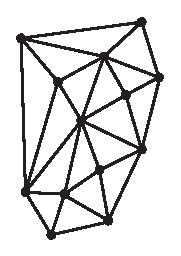
\includegraphics[width=\linewidth]{img/triangulation.eps}}
		\end{figure}
	\end{column}
	\begin{column}{0.7\textwidth} 
		Let the convex hull of a set $P$ of points defines a domain $\Omega$ in $\mathbb{R}^d$ 
		\bigskip
		
		The set of simplexes $\mathcal{T}_r$ is \alert{a triangulation} of $\Omega$ if
		\begin{itemize}
			\item The vertices of the elements in $ \mathcal{T}_r$ is exactly $P$.
			\item $ \Omega = \bigcup_{T \in \mathcal{T}_r}  T $.
			\item The intersection of the interior of any two elements is an empty set.
			\item The intersection of two elements in  $\mathcal{T}_r$ is either reduced to
				  the empty set or a vertex, an edge, or a face (for $d=3$ ).
		\end{itemize}
	\end{column}
\end{columns}
\end{frame}

\begin{frame}{Delaunay Triangulation}
\begin{columns}
	\begin{column}{0.4\textwidth} 
			\center{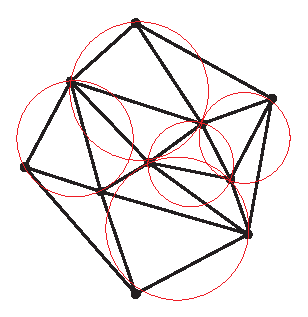
\includegraphics[width=\linewidth]{img/Delaunay.eps}}
		\end{column}
		\begin{column}{0.6\textwidth}
			A \alert{Delaunay triangulation $\mathcal{DT}_r$} of a set $P$ of points in a plane  
			is a triangulation such that no point in $P$ is inside the circumcircle of any
			triangle in $\mathcal{T}_r$  
		\end{column}
\end{columns}
\end{frame}

\begin{frame}{Delauney Triangulation Properties}
\begin{columns}
	\begin{column}{0.4\textwidth} 
			\center{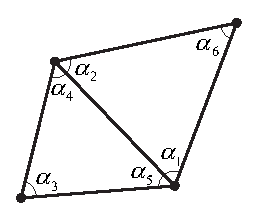
\includegraphics[width=\linewidth]{img/angle_triangulation.eps}}
		\end{column}
	\begin{column}{0.6\textwidth}
		An \alert{angle vector} of triangulation 
		$\mathcal{T}_r$ is $\mathcal{A}(\mathcal{T}_r)=(\alpha_1,...,\alpha_{3m})$
		where $\alpha_1,...,\alpha_{3m}$ are the angles of $\mathcal{T}_r$ 
		sorted by increasing value.
		\bigskip
			
		Any angle-optimal in a \alert{lexicographically} sense triangulation of $P$ 
		is a Delaunay triangulation of $P$.
		\bigskip
		
		Furthermore, any Delaunay triangulation of $P$ maximizes the minimum angle
		over all triangulations of $P$.
	\end{column}
\end{columns}
\end{frame}

\begin{frame}{Edge Flipping}
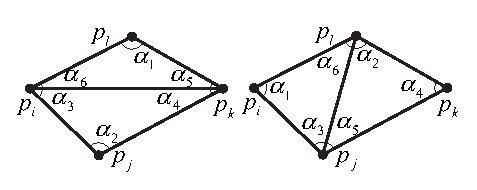
\includegraphics[width=\linewidth]{img/flip_triangle.eps}
	
	Flipping of an edge leads to changing in angle vector:
	
	$\alpha_1,...,\alpha_6$ are replaced by $\alpha_1',...,\alpha_6'$.

\end{frame}

\begin{frame}{Incremental Algorithm}
\begin{columns}
		\begin{column}{0.4\textwidth} 
			\center{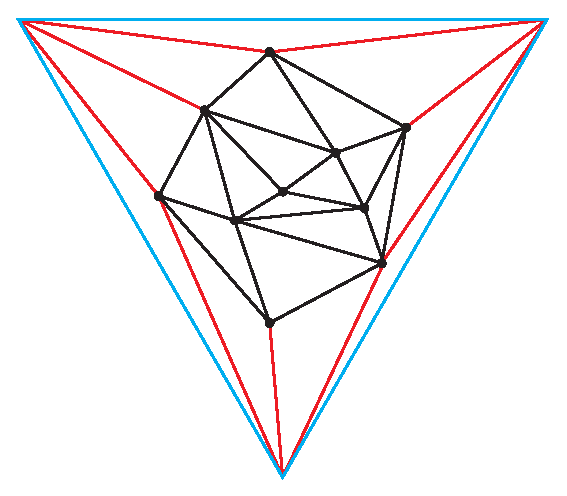
\includegraphics[width=\linewidth]{img/iterative.eps}}
		\end{column}
		\begin{column}{0.6\textwidth}
			\alert{Incremental triangulation} algorithms are based on sequential addition of points 
			to a triangulation.  
			\begin{itemize}
				\item \textit{Step 1} Build a \alert{super triangle} that contains $P$.
				\item \textit{Step 2} Add a point to the triangulation:
					\begin{itemize}
						\item Find triangle that contains the point.
						\item If the point lies on edge, divide two adjacent triangles into four parts.
						\item If the point lies in triangle interior, divide triangle into three parts.
						\item Improve triangulation.
					\end{itemize}
				\item \textit{Step 3} Remove triangles that contains the vertices of the super triangle.
			\end{itemize}
		\end{column}
	\end{columns} 
\end{frame}

\begin{frame}{Euclidean Graph}
\begin{columns}
	\begin{column}{0.4\textwidth} 
			\center{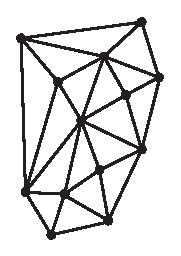
\includegraphics[width=\linewidth]{img/triangulation.eps}}
	\end{column}
	\begin{column}{0.6\textwidth}
		\alert{Planar graph} is a graph that can be embedded in the plain,
		i.e., it can be drawn on the plane in such a way that its edges
		intersect at their endpoints.
		\bigskip
		
		\alert{A Euclidean graph} is a planar graph in which the vertices are
		embedded as a points in the Euclidean plane, and the edges are embedded
		as non-crossing line segments. 
	\end{column}
\end{columns}
\end{frame}

\section{Voronoi Diagram}

\begin{frame}{Problem}
	\alert{Given} a set of point $P={p_1,..,i_n}$ and a point $p$  in a plane.
	\bigskip
	
	\alert{Goal.} Find the closest point $p_i$ to the given point $p$.
\end{frame}

\begin{frame}{Simple cases}
	\center{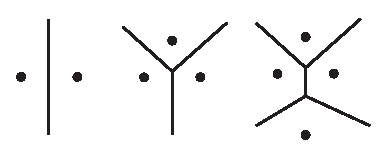
\includegraphics[width=\linewidth]{img/simple_voronoi.eps}}
\end{frame}



\begin{frame}{General case}
	\center{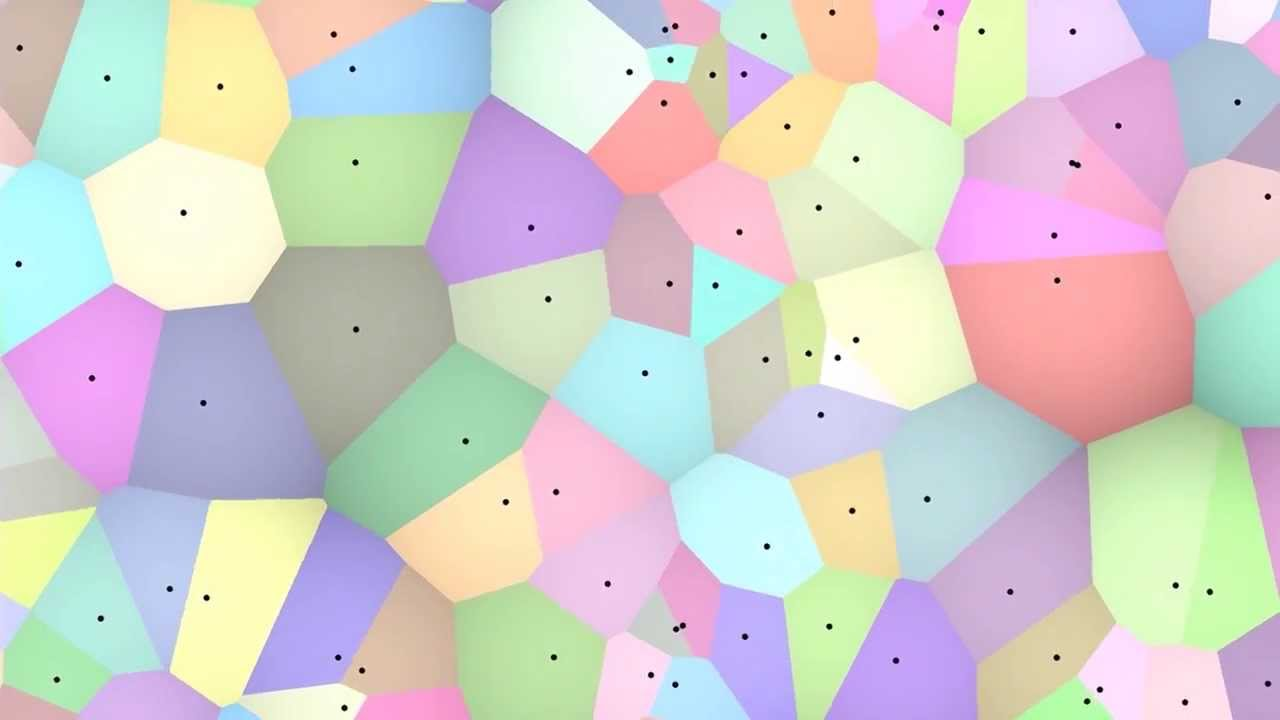
\includegraphics[width=\linewidth]{img/general_voronoi.jpg}}
\end{frame}


\begin{frame}{Voronoi Diargram}
	\alert{Voronoi diagram} of a set of point $P$ is a partitioning of a plane into 
	regions (tiles) $R_k$ that
	$$
		R_k =  \{x \in  \mathbb{R}^2 | d(x,p_k) \leq d(x,p_j) \forall j \neq k \}
	$$
	
	\alert{Dual graph} of a plane graph $G$ is a graph that has a vertex 
	for each face of $G$ and an edge whenever two faces of $G$ are separated 
	from each other by an edge, and self-loop when the same face appears on both
	sides of an edge.
	\bigskip
	
	The Voronoi diagram is a dual graph to a Delaunay triangulation with vertices 
	in a centers of circumcircles. 
\end{frame}


\section{Minimal Spanning Tree}

\begin{frame}{Minimum Spanning Tree}
\begin{columns}
		\begin{column}{0.4\textwidth} 
			\center{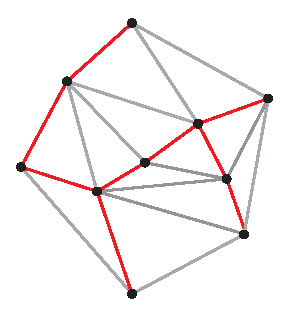
\includegraphics[width=\linewidth]{img/mst.eps}}
		\end{column}
		\begin{column}{0.6\textwidth}
			A \alert{Minimum spanning tree} is a subset of the edges of a connected,
			edge-weighted undirected graph that connects all the vertices together,
			without any cycles and with the minimum possible total edge weight.
		\end{column}
	\end{columns} 
\end{frame}

\begin{frame}{Algorithm}
	\alert{Prim's Algorithm}
	\begin{itemize}
		\item Init a tree with a single vertex, chosen arbitrarily from the graph.
		\item Grow the tree by one edge: of the edges that connect the tree to vertices 
			  not yet in the tree, find the minimum weight edge, and transfer it to the
			  tree.
	\end{itemize}
	\alert{Kruskal's algorithm}
	\begin{itemize}
		\item Create a forest $F$, where each vertex in the graph is a separate tree.
		\item Create a set $S$ containing all the edges in the graph.
		\item While $S$ is nonempty and $F$ is not yet spanning
			\begin{itemize}
				\item remove an edge with minimum weight from $S$,
				\item if the removed edge connects two different trees then add it to 
				the forest $F$, combining two trees into a single tree.
			\end{itemize}
	\end{itemize}
\end{frame}

\section{Pub Crawl Problem}

\begin{frame}
Given a set $P$ of points in the plane, the \alert{Euclidean Traveling
Salesperson Problem} is to compute a tour (cycle) that visits
all points of P and has minimum length.

A brute-force algorithm has a complexity $O(n!)$.

\end{frame}

\begin{frame}{Approximation algorithms}	

	If an algorithm A solves an optimization problem always
	within a factor k of the optimum, then A is called an
	\alert{$k$-approximation algorithm}.
	\bigskip
	
	If an instance I of ETSP has an optimal solution of length $L$,
	then a k-approximation algorithm will find a tour of length
	$\leq k \cdot L$.

\end{frame}

\begin{frame}{Visualization}
\center{
				\animategraphics[
						width = 0.9\linewidth ,					
						controls, loop
					]{1}{img/pcp_}{1}{13}
		}
\end{frame}

\end{document}